\documentclass[]{book}

\usepackage{array,epsfig}
\usepackage{amsxtra}
\usepackage{amsthm}
\usepackage{mathrsfs}
\usepackage{multirow}
\usepackage{float}
\usepackage{tabularray}
\usepackage[table]{xcolor}
\usepackage{hyperref} 
%Pagination stuff.
\setlength{\topmargin}{-.3 in}
\setlength{\oddsidemargin}{0in}
\setlength{\evensidemargin}{0in}
\setlength{\textheight}{9.in}
\setlength{\textwidth}{6.5in}
\pagestyle{empty}


\begin{document}


\begin{center}
{\Large Programmation linéaire:\\ Modélisation, Méthode graphique et méthode du simplexe}
\newline
\newline
\textbf{EL GHEMARY Farah}\\ 
Septembre 2025
\end{center}

\vspace{0.2 cm}



\section{Exercices}

\subsection*{Exercice 1:  Problème d’agriculture}
Un agriculteur veut allouer 150 hectares de surface irrigable entre culture de tomates et celles de piments. Il dispose de 480 heures de main d’œuvre et de 440 m3 d’eau. Un hectare de tomates demande 1 heure de main d’œuvre, 4 m3 d’eau et donne un bénéfice net de 100 dinars. Un hectare de piments demande 4 heures de main d’œuvre, 2 m3 d’eau et donne un bénéfice net de 200 dinars.
\\
Le bureau du périmètre irrigué veut protéger le prix des tomates et ne lui permet pas de cultiver plus de 90 hectares de tomates. Quelle est la meilleure allocation de ses ressources ? 

\subsection*{Exercice 2: Problème de médecine }
Un spécialiste en médecine a fabriqué un médicament (des pilules) pour guérir les sujets atteints d’un rhume. Ces pilules sont fabriquées selon deux formats :
\begin{itemize}
    \item Petite taille : elle contient 2 grains d’aspirine, 5 grains de bicarbonate et 1 grain de codéine.
    \item Grande taille : elle contient 1 grain d’aspirine, 8 grains de bicarbonate et 6 grains de codéine.
\end{itemize}
Pour guérir la maladie, le sujet a besoin de 12 grains d’aspirine, 74 grains de bicarbonate et 24 grains de codéine. Déterminer le nombre de pilules minimales à prescrire au sujet pour qu’il soit guérit.

\subsection*{Exercice 3: problème de production }
Pour fabriquer deux produits $P_1$ et $P_2$ on doit effectuer des opérations sur trois machines $M_1$, $M_2$ et $M_3$, successivement mais dans un ordre quelconque. Les temps unitaires d’exécution sont donnés par le tableau suivant :
\begin{center}
\begin{tabular}{ | m{1cm} | m{1cm}| m{1cm} | m{1cm} | } 
  \hline
    & $M_1$ & $M_2$ & $M_3$\\ 
    \hline
    $P_1$ & 11 mn & 7 mn & 6 mn\\  
    \hline
    $P_2$ & 9 mn & 12 mn & 16 mn\\
    \hline
\end{tabular}
\end{center}
On supposera que les machines n’ont pas de temps d’inactivité.
La disponibilité pour chaque machine sont :
\begin{itemize}
    \item 165 heures (9900 minutes) pour la machine $M_1$ ;
    \item 140 heures (8400 minutes) pour la machine $M_2$ ;
    \item 160 heures (9600 minutes) pour la machine $M_3$ .
\end{itemize}
Le produit $P_1$ donne un profit unitaire de 900 dinars et le produit $P_2$ un profit unitaire de 1000 dinars.
Dans ces conditions, combien doit-on fabriquer mensuellement de produits $P_1$ et $P_2$ pour avoir un profit total maximum ?


\subsection*{Exercice 4: Sélection de Médias }
Une entreprise désire effectuer une campagne publicitaire dans la télévision, la radio et les journaux pour un produit lancé récemment sur le marché. Le but de la campagne est d’attirer le maximum possible de clients. Les résultats d’une étude de marché sont donnés par le tableau suivant :\\
\begin{center}
    \begin{tabular}{ |p{5cm}||p{2cm}|p{2cm}|p{2cm}|p{2cm}|p{2cm}| }
        \hline
        & \multicolumn{2}{c|}{Télévision} & \multirow{2}{*}{Radio} & \multirow{2}{*}{Journaux} \\ 
        \cline{2-3}
        & Locale & Par satellite &  &  \\ 
        \hline \hline
        Coût d'une publicité & 40 DT & 75 DT& 30 DT & 15 DT \\
        \hline
        Nombre de client potentiel par publicité & 400 & 900& 500 & 200 \\
        \hline
        Nombre de client potentiel femme par publicité & 300& 400 & 200 & 100 \\
        \hline
    \end{tabular}
\end{center}
Pour la campagne, on prévoit de ne pas payer plus que 800DT pour toute la campagne et on demande que ces objectifs soient atteints :
\begin{itemize}
    \item Au minimum 2000 femmes regardent, entendent ou lisent la publicité ;
    \item La campagne publicitaire dans la télévision ne doit pas dépasser 500 DT ;
    \item Au moins 3 spots publicitaires seront assurer par la télévision locale et au moins de deux spots par la télévision par satellite.
    \item Le nombre des publicités dans la radio ou dans les journaux sont pour chacun entre 5 et 10.
\end{itemize}

\subsection*{Exercice 5: PL}
    $Max$ $Z(x_1,x_2) = 2x_1 + 4x_2$\\
s/c $\left\{
	\begin{array}l
	x_1 + 3x_2 \leq 18\\
    x_1 + x_2 \leq 8\\
    2x_1 + x_2 \leq 14\\
	x_1 \geq 0, x_2 \geq 0\end{array}
	\right.$

\subsection*{Exercice 6: PL}
    $Max$ $z(x_1,x_2) = 6x_1 + 4x_2$\\
s/c $\left\{
	\begin{array}l
	3x_1 + 9x_2 \leq 81\\
    4x_1 + 5x_2 \leq 55\\
    2x_1 + x_2 \leq 20\\
	x_1 \geq 0, x_2 \geq 0\end{array}
	\right.$
 \section{Méthode Graphique}
   
\subsection*{Correction 1}
\subsubsection{Formulation en un Problème linéaire}
\underline{Les variables de décision:}
\begin{itemize}
    \item $x_1$: Surface de Tomates.
    \item $x_2$: Surface de piments.
\end{itemize}
Les contraintes de non-négativité sont vérifiées.\\\\
\underline{Les contraintes du problème :}
\begin{itemize}
    \item main d’œuvre: $ x_1 + 4x_2 \leq 480$
    \item volume d'eau : $ 4x_1 + 2 x_2\leq 440$
    \item Surface totale: $x_1 + x_2 \leq 150 $
    \item limitation de tomates $x_1 \leq 90$
    \item $x_1 \geq 0, x_2 \geq 0$
\end{itemize}
\underline{La fonction objectif:}
maximiser le profit avec les même ressources 

\begin{center}
    $z = 100 x_1 + 200 x_2$
\end{center}
\underline{Le programme linéaire} qui modélise le problème d’agriculture est :
\begin{center}
    $Max$ $Z(x_1,x_2) = 100 x_1 + 200 x_2$\\
s/c $\left\{
	\begin{array}l
	x_1 + 4x_2 \leq 480\\
    4x_1 + 2 x_2\leq 440\\
    x_1 + x_2 \leq 150\\
	x_1 \leq 90\\
    x_1 \geq 0, x_2 \geq 0\end{array}
	\right.$
\end{center} 
\subsubsection{Solution Graphique:}
\underline{L'ensemble des solutions réalisables:}

Soit les droites d'équations suivantes:
\begin{center}
    $(D_1): x_1 + 4x_2 = 480$, $(D_2): 4x_1 + 2 x_2 = 440$, $(D_3): x_1 + x_2 = 150$ et $(D_4): x_1 = 90$
\end{center}
\begin{center}
    \begin{tabular}{ | m{0.5cm} | m{0.5cm}| m{1cm} | m{1cm} | } 
      \hline
        \multirow{2}{4em}{$D_1$} & $x_1$  & 0 & 80 \\
        \cline{2-4} & $x_2$  & 120 & 100 \\
        \hline
        
        \multirow{2}{4em}{$D_2$} & $x_1$ & 110 & 100 \\
        \cline{2-4} & $x_2$ & 0 & 20 \\
        \hline
        
        \multirow{2}{4em}{$D_3$} & $x_1$ & 0 & 150 \\
        \cline{2-4} & $x_2$ & 150 & 0 \\
        \hline
    \end{tabular}
\end{center}

\underline{La solution Optimale:}

\begin{figure}[H]
    \centering
    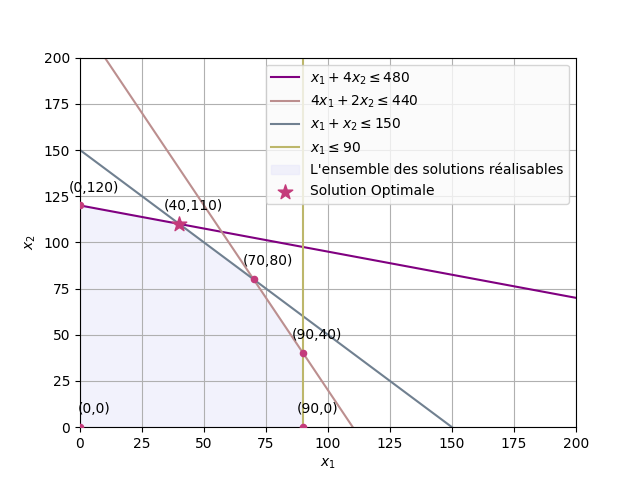
\includegraphics[width=0.6\textwidth]{Figures/figure_01.png}
    \caption{Représentation Graphique de l'ensemble des solutions réalisables}
    \label{fig:placeholder}
\end{figure}
\newpage
La fonction objectif $max$ $z = 100 x_1 + 200 x_2$ est une droite linéaire\\
Déterminons les couples $(x_1, x_2)$ solutions réalisables tq $Z(x_1,x_2) = 100 x_1 + 200 x_2$ soit maximum\\
On note $D_z$ la droite d'isovaleur de la fonction objectif tq $Z = 100 x_1 + 200 x_2$\\
son vecteur est $\Vec{v}(-2,1)$ et son coefficient directeru est $\frac{-1}{2}$\\
La solution optimale est $(x_1,x_2)=(40,110)$, et ce qui donne une valeur maximale de $max(Z(x_1,x_2)) = 26000$

\subsection*{Correction 2}
\subsubsection{Formulation en un problème linéaire:}
\underline{Les variables de décision:}
\begin{itemize}
    \item $x_1:$ Nombre de pilules petit format
    \item $x_2:$ Nombre de pilules grand format
\end{itemize}
Les contraintes de non-négativité sont vérifiées\\
\underline{Les contraintes:}
\begin{itemize}
    \item Aspirine: $2x_1+x_2 \geq 12$
    \item Bicarbonate: $5x_1 + 8x_2 \geq 74$
    \item Codéine: $x_1 + 6x_2 \geq 24$
    \item $x_1 \geq 0$, $x_2 \geq 0$
\end{itemize}
\underline{La fonction objectif:}
Minimiser le nombre de pilules à prescrire\\
\begin{center}
    $Z(x_1,x_2) = x_1 + x_2$
\end{center}
\underline{Le problème linéaire}
\begin{center}
    $\min$ $Z(x_1,x_2) = x_1 + x_2$\\
s/c $\left\{
	\begin{array}l
	2x_1 + x_2 \geq 12\\
    5x_1 + 8 x_2 \geq 74\\
    x_1 + 6x_2 \geq 24\\
    x_1 \geq 0, x_2 \geq 0\end{array}
	\right.$
\end{center} 

\subsubsection{Solution Graphique:}
\underline{L'ensemble des solutions réalisables:}\\
Soit les droites d'équations suivantes:
\begin{center}
    $(D_1): 2x_1 + x_2 = 12$, $(D_2): 5x_1 + 8 x_2 = 74$, $(D_3): x_1 + 6x_2 = 24$, 
\end{center}

\begin{center}
    \begin{tabular}{ | m{0.5cm} | m{0.5cm}| m{1cm} | m{1cm} | } 
      \hline
        \multirow{2}{4em}{$D_1$} & $x_1$  & 0 & 6 \\
        \cline{2-4} & $x_2$  & 12 & 0 \\
        \hline
        
        \multirow{2}{4em}{$D_2$} & $x_1$ & 0 & $\frac{74}{5}$ \\
        \cline{2-4} & $x_2$ & $\frac{37}{4}$ & 0 \\
        \hline
        
        \multirow{2}{4em}{$D_3$} & $x_1$ & 0 & 6 \\
        \cline{2-4} & $x_2$ & 4 & 3 \\
        \hline
    \end{tabular}
\end{center}


\underline{La solution Optimale:}

\begin{figure}[H]
    \centering
    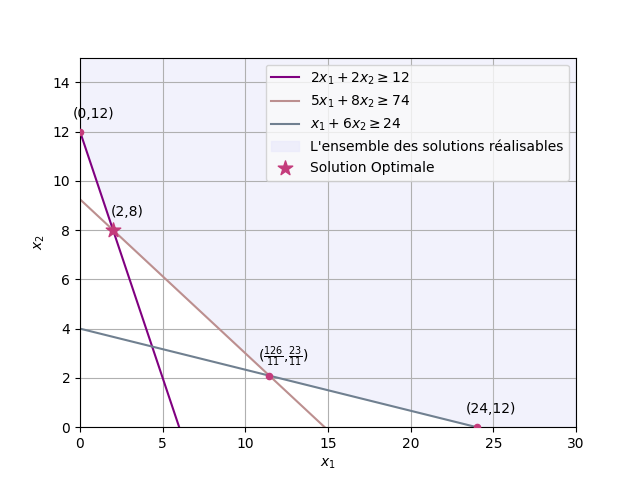
\includegraphics[width=0.7\textwidth]{Figures/figure_02.png}
    \caption{Représentation Graphique de l'ensemble des solutions réalisables}
    \label{fig:placeholder}
\end{figure}

La fonction objectif $\min$ $Z(x_1,x_2) = x_1 + x_2$ est une droite linéaire\\
Déterminons les couples $(x_1, x_2)$ solutions réalisables tq $Z(x_1,x_2) = x_1 + x_2$ soit minimum\\
On note $D_z$ la droite d'isovaleur de la fonction objectif tq $Z = x_1 + x_2$\\
son vecteur est $\Vec{v}(-1,1)$ et son coefficient directeur est $-1$\\
La solution optimale est $(x_1,x_2)=(2,8)$, et ce qui donne une valeur minimale de $min(Z(x_1,x_2)) = 10$


\subsection*{correction 3}
\subsubsection{Formulation en un problème linéaire:}
\underline{Les variables de décision:}
\begin{itemize}
    \item $x_1:$ Nombre de fabrication mensuelle de produit $P_1$ 
    \item $x_2:$ Nombre de fabrication mensuelle de produit $P_2$ 
\end{itemize}
Les contraintes de non-négativité sont vérifiées\\
\underline{Les contraintes:}
\begin{itemize}
    \item Machine $M_1$: $11 x_1 + 9 x_2 \leq 9900$
    \item Machine $M_2$ $ 7x_1 + 12 x_2 \leq 8400$
    \item Machine $M_3$: $6 x_1 + 16 x_2 \leq 9600$
    \item $x_1 \geq 0$, $x_2 \geq 0$
\end{itemize}
\underline{La fonction objectif:}
Maximiser le profit\\
\begin{center}
    $Z(x_1,x_2) = 900 x_1 + 1000 x_2$
\end{center}
\underline{Le problème linéaire}
\begin{center}
    $\max Z(x_1,x_2) = 900 x_1 + 1000 x_2$\\
s/c $\left\{
	\begin{array}l
	11 x_1 + 9 x_2 \leq 9900\\
    7x_1 + 12 x_2 \leq 8400\\
    6 x_1 + 16 x_2\leq 9600\\
    x_1 \geq 0, x_2 \geq 0\end{array}
	\right.$
\end{center} 

\subsubsection{Solution Graphique:}
\underline{L'ensemble des solutions réalisables:}\\
Soit les droites d'équations suivantes:
\begin{center}
    $(D_1): 11 x_1 + 9 x_2 = 9900$, $(D_2): 7x_1 + 12 x_2 = 8400$, $(D_3): 6 x_1 + 16 x_2 = 9600$, 
\end{center}

\begin{center}
    \begin{tabular}{ | m{0.5cm} | m{0.5cm}| m{1cm} | m{1cm} | } 
      \hline
        \multirow{2}{4em}{$D_1$} & $x_1$  & 0 & 900 \\
        \cline{2-4} & $x_2$  & 1100 & 0 \\
        \hline
        
        \multirow{2}{4em}{$D_2$} & $x_1$ & 0 & 1200 \\
        \cline{2-4} & $x_2$ & 700 & 0 \\
        \hline
        
        \multirow{2}{4em}{$D_3$} & $x_1$ & 0 & 1600 \\
        \cline{2-4} & $x_2$ & 600 & 0\\
        \hline
    \end{tabular}
\end{center}

\underline{La solution Optimale:}
\begin{figure}[H]
    \centering
    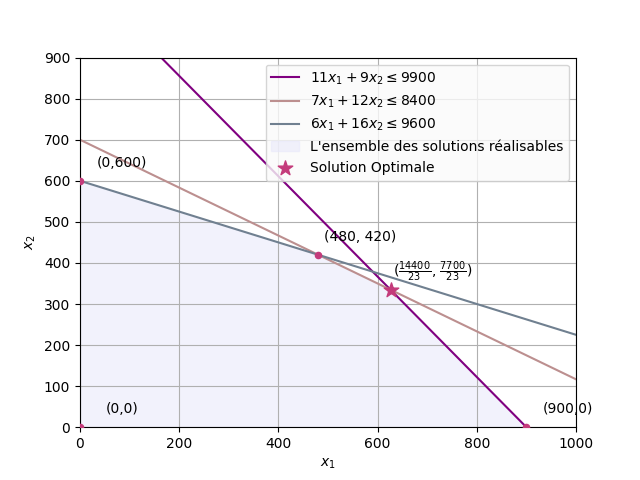
\includegraphics[width=0.7\textwidth]{Figures/figure_03.png}
    \caption{Représentation Graphique de l'ensemble des solutions réalisables}
    \label{fig:placeholder}
\end{figure}
La fonction objectif $\max$ $Z(x_1,x_2) = 900x_1 + 1000x_2$ est une droite linéaire\\
Déterminons les couples $(x_1, x_2)$ solutions réalisables tq $Z(x_1,x_2) = 900x_1 + 1000x_2$ soit maximum\\
On note $D_z$ la droite d'isovaleur de la fonction objectif tq $Z = 900x_1 + 1000x_2$\\
son vecteur est $\Vec{v}(-10,9)$ et son coefficient directeur est $-0.9$\\
La solution optimale est $(x_1,x_2)=(\frac{14400}{23},\frac{7700}{23})$, et ce qui donne une valeur minimale de $min(Z(x_1,x_2)) = 898260.8696$






\subsection*{Correction 4}
\subsubsection{Formulation en un problème linéaire:}
\underline{Les variables de décisions:}
\begin{itemize}
    \item $x_1:$ Nombre de publicités dans la Télévision locale
    \item $x_2:$ Nombre de publicités dans la Télévision par satellite
    \item $x_1:$ Nombre de publicités dans la Radio
    \item $x_2:$ Nombre de publicités dans les Journaux
\end{itemize}
Les contraintes de non-négativité sont vérifiées\\\\
\underline{Les contraintes:}
\begin{itemize}
    \item Budget de campagne publicitaire: $40 x_1 + 75 x_2 + 30 x_3 + 15 x_4 \leq 800$
    \item Nombre de clients femmes: $300 X_1 + 400 x_2 + 200 x_3 + 100 X_4 \geq 200$
    \item nombre de spots publicitaires assurer par la télévision locale: $x_1 \geq 3$
    \item nombre de spots publicitaires assurer par la télévision par satéllite: $x1 \geq 2$
    \item nombre des publicités dans la radio: $ 5 \leq x_3 \leq 10 $
    \item nombre des publicités dans les journaux: $ 5 \leq x_4 \leq 10 $
    \item $x_1 \geq 0$, $x_2 \geq 0$, $x_3 \geq 0$, $x_4 \geq 0$, 
\end{itemize}
\underline{La fonction objectif:}
Maximiser les clients
\begin{center}
    $z(x_1,x_2) = 400 x_1 + 900 x_2 + 500 x_3 + 200 x_4$
\end{center}
\underline{Le problème linéaire}
\begin{center}
    $\max z(x_1,x_2) = 400 x_1 + 900 x_2 + 500 x_3 + 200 x_4$\\
s/c $\left\{
	\begin{array}l
	40 x_1 + 75 x_2 + 30 x_3 + 15 x_4 \leq 800\\
    300 X_1 + 400 x_2 + 200 x_3 + 100 X_4 \geq 200\\
    x_1 \geq 3 \\
    x_2 \geq 2 \\
    x_3 \leq 10 \\
    x_3 \geq 5 \\
    x_4 \leq 10 \\
    x_4 \geq 5 \\
    x_1 \geq 0, x_2 \geq 0, x_3 \geq 0, x_4 \geq 0\end{array}
	\right.$
\end{center} 

Soit les droites d'équations suivantes:
\begin{center}

	$(D_1): 40 x_1 + 75 x_2 + 30 x_3 + 15 x_4 = 800$\\
    $(D_2): 300 X_1 + 400 x_2 + 200 x_3 + 100 X_4 = 200$\\
    $(D_3): x_1 = 3$, $(D_4): x_2 = 2$\\
    $(D_5): x_3 = 10$, $D_5): x_3 = 5$\\
    $(D_6): x_4 = 10$, $(D_7): x_4 = 5$\\
\end{center}
\subsubsection{Solution Graphique:}
Ce problème comporte plus de deux variables de décision. Dans ce cas, il n’est pas possible de représenter graphiquement l’ensemble des solutions réalisables dans un plan.
\subsection*{Correction 5}
\subsubsection{Programme linéaire:}
$Max$ $Z(x_1,x_2) = 2x_1 + 4x_2$\\
s/c $\left\{
	\begin{array}l
	x_1 + 3x_2 \leq 18\\
    x_1 + x_2 \leq 8\\
    2x_1 + x_2 \leq 14\\
	x_1 \geq 0, x_2 \geq 0\end{array}
	\right.$
\subsubsection{solution graphique}
Soit les droites d’´équations suivantes:
\begin{center}
    $(D_1): x_1 + 3 x_2 = 18$, $(D_2): x_1 + x_2 = 8$, $(D_3): 2 x_1 + x_2 = 14 $
\end{center}

\begin{center}
    \begin{tabular}{ | m{0.5cm} | m{0.5cm}| m{1cm} | m{1cm} | } 
      \hline
        \multirow{2}{4em}{$D_1$} & $x_1$  & 0 & 6 \\
        \cline{2-4} & $x_2$  & 6 & 4 \\
        \hline
        
        \multirow{2}{4em}{$D_2$} & $x_1$ & 0 & 8 \\
        \cline{2-4} & $x_2$ & 8 & 0 \\
        \hline
        
        \multirow{2}{4em}{$D_3$} & $x_1$ & 0 & 7 \\
        \cline{2-4} & $x_2$ & 14 & 0\\
        \hline
    \end{tabular}
\end{center}

\underline{La solution Optimale:}
\begin{figure}[H]
    \centering
    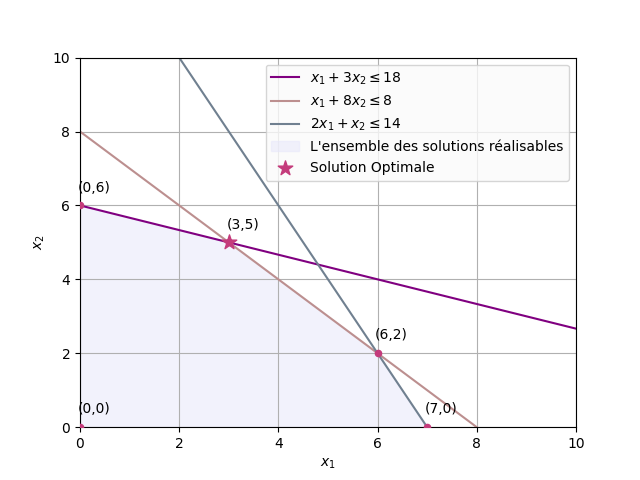
\includegraphics[width=0.7\textwidth]{Figures/figure_05.png}
    \caption{Représentation Graphique de l'ensemble des solutions réalisables}
    \label{fig:placeholder}
\end{figure}

La fonction objectif $\max$ $Z(x_1,x_2) = 2x_1 + 4x_2$ est une droite linéaire\\
Déterminons les couples $(x_1, x_2)$ solutions réalisables tq $Z(x_1,x_2) = 2 + 4x_2$ soit maximum\\
On note $D_z$ la droite d'isovaleur de la fonction objectif tq $Z = 2x_1 + 4x_2$\\
son vecteur est $\Vec{v}(-2,1)$ et son coefficient directeur est $\frac{-1}{2}$\\
La solution optimale est $(x_1,x_2)=(3,5)$, et ce qui donne une valeur minimale de $min(Z(x_1,x_2)) = 26 $


\subsection*{Correction 6}
\subsubsection{Programme linéaire}
    $Max$ $z(x_1,x_2) = 6x_1 + 4x_2$\\
s/c $\left\{
	\begin{array}l
	3x_1 + 9x_2 \leq 81\\
    4x_1 + 5x_2 \leq 55\\
    2x_1 + x_2 \leq 20\\
	x_1 \geq 0, x_2 \geq 0\end{array}
	\right.$
\subsubsection{Solution graphique}
Soit les droites d’équations suivantes:
\begin{center}
    $(D_1): 3x_1 + 9x_2 = 81$, $(D_2): 4x_1 + 5x_2 = 55$, $(D_3): 2x_1 + x_2 = 20$
\end{center}

\begin{center}
    \begin{tabular}{ | m{0.5cm} | m{0.5cm}| m{1cm} | m{1cm} | } 
      \hline
        \multirow{2}{4em}{$D_1$} & $x_1$  & 0 & 27 \\
        \cline{2-4} & $x_2$  & 9 & 0 \\
        \hline
        
        \multirow{2}{4em}{$D_2$} & $x_1$ & 0 & 10 \\
        \cline{2-4} & $x_2$ & 11 & 5 \\
        \hline
        
        \multirow{2}{4em}{$D_3$} & $x_1$ & 0 & 10 \\
        \cline{2-4} & $x_2$ & 20 & 0\\
        \hline
    \end{tabular}
\end{center}

\underline{La solution Optimale:}
\begin{figure}[H]
    \centering
    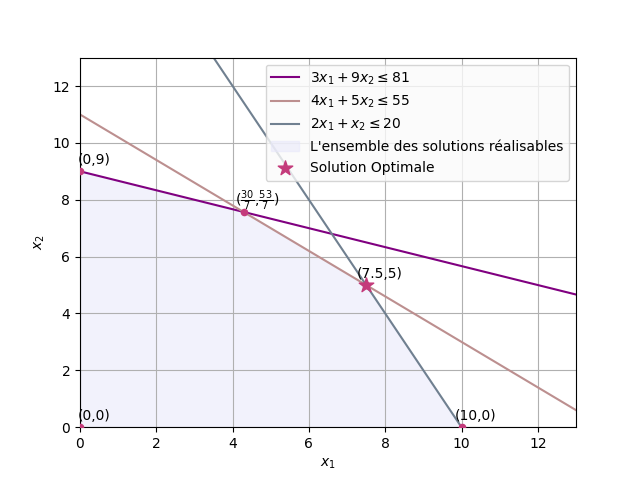
\includegraphics[width=0.7\textwidth]{Figures/figure_06.png}
    \caption{Représentation Graphique de l'ensemble des solutions réalisables}
    \label{fig:placeholder}
\end{figure}

La fonction objectif $\max$ $Z(x_1,x_2) = 6x_1 + 4x_2$ est une droite linéaire\\
Déterminons les couples $(x_1, x_2)$ solutions réalisables tq $Z(x_1,x_2) = 6x_1 + 4x_2$ soit maximum\\
On note $D_z$ la droite d'isovaleur de la fonction objectif tq $Z = 6x_1 + 4x_2$\\
son vecteur est $\Vec{v}(-2,3)$ et son coefficient directeur est $\frac{-3}{2}$\\
La solution optimale est $(x_1,x_2)=$, et ce qui donne une valeur minimale de $min(Z(x_1,x_2)) =  $

\appendix
\section*{Annexe : Code Source sur GitHub}

Tous les codes utilisés sont disponibles sur:

\begin{center}
\href{https://github.com/elghemary/MID-math-2025/tree/main/Recherche%20Operationnelle}{\texttt{Github Repository}}
\end{center}

Ce repository contient :
\begin{itemize}
    \item Les scripts \texttt{Python}.
    \item Les fichiers \LaTeX{}.
    \item Les figures.
\end{itemize}

\end{document}


